\section{Empirical Specification}
\subsection{Model Implementation}
The empirical analysis proceeds by implementing the theoretical models using the historical data. The process involves the following steps:
\begin{enumerate}
    \item \textbf{Data Cleaning and Preparation}: Ensuring the data is free from errors, outliers, and missing values. Adjustments are made for stock splits and dividends to maintain consistency in the price data.
    \item \textbf{Calculation of Daily Returns}: Daily returns are computed as the percentage change in closing prices, which serves as the basis for further analysis.
    \item \textbf{Estimation of Expected Returns and Variances}: Using historical data, the expected returns and variances for each asset are estimated. These estimates are inputs for the portfolio optimization process.
    \item \textbf{Portfolio Optimization}: Applying Modern Portfolio Theory to construct efficient portfolios that maximize expected return for a given level of risk. The optimization problem is solved using quadratic programming.
    \item \textbf{Simulation of Investment Scenarios}: Using Monte Carlo simulations to model the accumulation of down payments over different investment horizons. Multiple scenarios are simulated to capture the range of possible outcomes.
\end{enumerate}

\subsection{CAPM and Sharpe Ratio Calculation}
For each security, the Capital Asset Pricing Model (CAPM) and Sharpe Ratio are calculated. The CAPM is used to estimate the expected return of each security, while the Sharpe Ratio measures the risk-adjusted return. The steps involved are:
\begin{enumerate}
    \item Calculate the average return of the market index (e.g., a broad market index like the S\&P 500).
    \item Determine the risk-free rate (e.g., the yield on 10-year U.S. Treasury bonds).
    \item Compute the beta ($\beta$) of each security by regressing its returns against the market returns.
    \item Use the CAPM formula to estimate the expected return for each security.
    \item Calculate the Sharpe Ratio using the formula:
    \[
    S = \frac{E(R_i) - R_f}{\sigma_i}
    \]
    where \( E(R_i) \) is the expected return, \( R_f \) is the risk-free rate, and \( \sigma_i \) is the standard deviation of the security’s excess return.
\end{enumerate}

The securities are then ranked by their Sharpe Ratios to identify those with the best risk-adjusted returns.

\subsection{Modern Portfolio Theory (MPT) Application}
Using the ranked securities, portfolios are constructed for different age groups (5, 10, and 15 years from the average first-time homebuyer age of 35). Modern Portfolio Theory (MPT) is applied to optimize these portfolios, balancing the trade-off between risk and return. The steps include:
\begin{enumerate}
    \item Define the assets and their expected returns and covariances.
    \item Determine the weights of the assets in the portfolio to maximize the expected return for a given level of risk.
    \item Construct the efficient frontier to visualize the optimal portfolios.
\end{enumerate}

\subsection{Monte Carlo Simulation for Down Payment Accumulation}
Monte Carlo simulations are conducted to assess the variability and uncertainty in the investment returns. This involves generating random returns based on historical distributions and running numerous simulations to build a probability distribution of potential outcomes. The simulation process helps in understanding the range of possible values for the investment portfolio and the likelihood of achieving the target down payment within the specified timeframe.

\subsubsection{Simulation Process}
The simulation process involves the following steps:
\begin{enumerate}
    \item Define the initial investment amount and the annual contribution based on age-specific income data.
    \item Generate a series of random returns for each asset in the portfolio using historical return distributions.
    \item Compute the investment value at each time step by applying the generated returns.
    \item Repeat the simulation for a large number of iterations to obtain a distribution of possible outcomes.
    \item Analyze the distribution to determine the probability of achieving the down payment target.
\end{enumerate}

\begin{figure}[h]
\centering
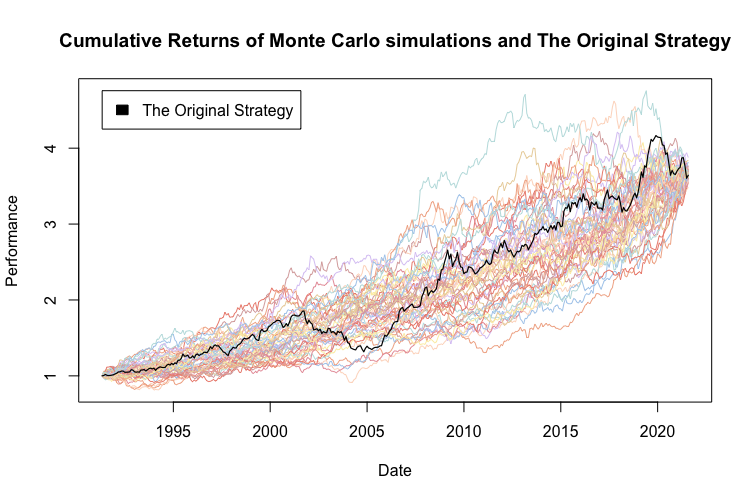
\includegraphics[width=0.5\textwidth]{investment_simulation_process.png}
\caption{Investment Simulation Process for Monte Carlo Analysis. Source: \href{https://quantpedia.com/introduction-and-examples-of-monte-carlo-strategy-simulation/}{Quantpedia}}
\label{fig:simulation_process}
\end{figure}

